\section{Appendix: Language Models} \label{sec:LanguageModels} % todo rename this from sec: to app: but problem is then would have to change it everywhere. 

A language model takes a sequence of word vectors and outputs a sequence of predicted word vectors by learning a probability distribution over words in a vocabulary. In representation terms, the ``vector representation of a word depends on the context vector representation" (Ibrahim, 2019). Many tasks such as \nameref{nlptask:machinetranslationMT}, spell correction, text summarization, \nameref{nlptask:questionansweringQA}, and \nameref{nlptask:sentimentanalysisSA} all use language models to convert text into machine-interpretable language (Chromiak, 2017). 

Intuitively, language models predict words in a blank. For instance, given the following context: ``The $\_\_\_$ sat on the mat" where $\_\_\_$ is the word to predict, a language model might suggest the word ``cat" should fill the blank a certain percentage of the time and the word ``dog" would fill the blank with lower probability (Kurita, 2019). 

Formally, language models compute the conditional probability of a word $w_t$ given a context, such as its previous $n-1$ words: $P(w_t | w_{t-1}, ..., w_{t-n+1})$ (Ruder, 2016). The joint probability of a $T$-sized sequence of word tokens $w_1, ..., w_T$ from a sentence $S$ is expressed as:

\begin{equation}
\begin{array}{ll}
P(S)
&= P \Big(w_1, ..., w_T \Big)  \\
&= P(w_1) \cdot P(w_2 \; | \; w_1) \cdot ... \cdot P(w_n \; | \; w_1, ..., w_{T-1}) \\
&= \prod_{t=1}^T P \Big(w_t \; | \; w_1, ..., w_{t-1} \Big) \\
\end{array}
\label{eq:LangModelProduct}
\end{equation}

Typically, the \textbf{Markov Assumption}, which states that the probability of a word depends only on its previous word, reduces context history and intake of model data. Thus the joint probability in \cref{eq:LangModelProduct} is estimated using the $n$ previous words as: $P \Big(w_1, ..., w_T \Big) \approx \prod_{t=1}^T P \Big(w_t \; | \; w_{t-1}, ..., w_{t-n+1} \Big)$.



\subsection{$n$-gram language model} \label{sec:NGramLM}

An $n$-gram is a sequence of $n$ words. The simple $n$-gram language model assigns probabilities to sentences and word sequences. It calculates a word's probability based on the frequencies of its constituent $n$-grams, taking just the preceding $n-1$ words as context instead of the entire corpus (Ruder, 2016): $P \Big(w_t \; | \; w_{t-1}, ..., w_{t-n+1} \Big) = \frac {count(w_{t-n+1},...,w_{t-1},w_t)} {count(w_{t-n+1},...,w_{t-1})}$

%\begin{equation}

%\label{eq:NGramEq}
%\end{equation}

\subsection{neural network language model} \label{sec:NeuralLM}


\subsubsection{Curse of Dimensionality} \label{sec:CurseDim}

Bengio et al. (2003) defines the \emph{curse of dimensionality} in NLP as how a word sequence may differ from the training set of word sequences. This appears when modeling the joint distribution between discrete random variables (like words in a sentence). 

\subsubsection{Key Concept: Neural Network Representation} \label{sec:NeuralNetRepr}

A \textbf{neural network} is a function from vectors to vectors. All neural network representations rely on a structure called a neuron, a linear formula: $W \cdot x + b$. By applying a nonlinear function $f(\cdot)$ to the neuron and by incorporating many hidden layers and by stacking neurons together, a neural network can model any function. %A neuron is shown in %\cref{fig:neuronPic}.

Many \hyperref[app:Appendix_NLPTasks]{NLP applications} using neural networks feed in word tokens as parameters that are \emph{optimized} to fit text by minimizing a continuous loss function (Smith, 2019). There are three components to a neural network: 

\begin{enumerateSpaced}{4pt}
    \item \textbf{Embedding Layer}\label{cnc:embeddingLayer}: this layer creates word embeddings by multiplying an index vector with a word vector matrix. 
    
    \item \textbf{Intermediate Layer(s)}: multiple layers are used to create a fully-connected layer that applies a non-linearity function (like hyperbolic tangent or sigmoid) to the concatenation of word embeddings. 
    
    \item \textbf{Softmax Layer}\label{cnc:softmaxLayer}: the last layer normalizes the word embedding matrix to using a \textbf{softmax function} to create a probability distribution over words $w_t$ in the vocabulary: $P \Big(w_t \; | \; w_{t-1}, ..., w_{t-n+1} \Big) = \frac {\exp{ \Big(h^T \cdot v_{w_t}' \Big) }} {\sum_{w_i \in V} \exp{ \Big(h^T \cdot v_{w_i}' \Big) }}$, where $V = $ vocabulary of a corpus, $h = $ output vector of the hidden layer, and $v_w' = $ the output embedding of word $w$. 
    %$$
    %P \Big(w_t \; | \; w_{t-1}, ..., w_{t-n+1} \Big) = \frac {\exp{ \Big(h^T \cdot v_{w_t}' \Big) }} {\sum_{w_i \in V} \exp{ \Big(h^T \cdot v_{w_i}' \Big) }}
    %$$
    
\end{enumerateSpaced}

%Many neural networks are \textbf{feed-forward neural network (FNN)}\label{cnc:ffn}s, in which input is fed in the forward direction only. 


\subsubsection{Solution to Curse of Dimensionality: Neural Model and Continuous Vector Representations} \label{sec:SolutionToCurseDim}

The $n$-gram model seeks to remedy the \emph{curse of dimensionality} by combining short overlapping word sequences seen in the training set. 

However, Bengio et al. (2003) developed a \emph{neural probabilistic language model} to learn a \hyperref[sec:DistributedRepr]{distributed representation} for words to allow the model to generalize to unseen data. The neural model does two tasks simultaneously; (1) it learns a \hyperref[sec:DistributedRepr]{distributed representation} for each word, and also (2) it learns the probability distribution of word sequences \emph{as a function of} the \hyperref[sec:DistributedRepr]{distributed representations}. Since the neural model uses continuous word vector representations, the learned probability function's parameters increase linearly, rather than exponentially, with the vocabulary size and vector dimension, thus resolving the curse of dimensionality (Bengio et al., 2003).  

%The neural model can capture longer contexts as opposed to the \hyperref[sec:NGramLM]{$n$-gram model}. 





\subsection{bidirectional language model (biLM)} \label{sec:BidirectionalLM}

\subsubsection{forward language model} \label{sec:ForwardLM}

A general language model predicts a next word given its context words, $P(\textit{Word} \: | \: \textit{Context})$. 

A \textbf{forward language model} takes this context to be previous words. From Peters et al. (2018), given a sequence of $N$ tokens $(t_1, t_2, ..., t_N)$, a forward language model calculates the probability of the tokenized sentence assuming the probability of a word token $t_k$ is conditional on its history tokens: $P \Big(t_1, t_2, ..., t_N \Big) = \prod_{k=1}^N P \Big(t_k \; | \; t_1, t_2, ..., t_{k-1} \Big)$.

\subsubsection{backward language model} \label{sec:BackwardLM}

A \textbf{backward language model} is similar to a forward model excepts it predicts the current token $t_k$ conditional on future context tokens: $P \Big(t_1, t_2, ..., t_N \Big) = \prod_{k=1}^N P \Big(t_k \; | \; t_{k+1}, t_{k+2}, ..., t_N \Big)$.

\subsubsection{Combining Forward and Backward}

A \textbf{bidirectional language model (biLM)} combines the \hyperref[sec:ForwardLM]{forward} and \hyperref[sec:BackwardLM]{backward language model}s during maximum likelihood estimation to \emph{jointly} maximize the log likelihood of the forward and backward directions: 
\begin{equation}
\sum_{k=1}^N \Big( \text{log} \Big( P \Big(t_k \; | \; t_1,...,t_{k-1}; \; \overrightarrow{\theta} \Big) + \text{log} \Big( P \Big(t_k \; | \; t_{k+1}, t_{k+2}, ..., t_N; \; \overrightarrow{\theta} \Big) \Big)
\label{eq:BiLMLoss}
\end{equation}
where $\overrightarrow{\theta}$ represents additional parameters (Peters et al., 2018). 


% \begin{figure}[h]
% \vspace{-5pt}
% \centering
% 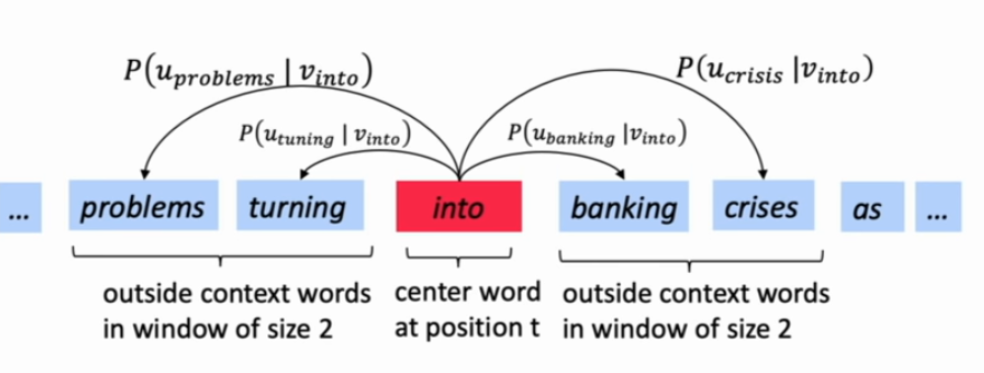
\includegraphics[width=0.6\textwidth]{bidirectional_languagemodel_banking.png}
% \vspace{-5pt}
% \caption{\footnotesize Example Bidirectional Language Model. From \emph{Word2Vec Overview With Vectors}, by CS224n: Natural Language Processing with Deep Learning (Stanford), 2018. \url{https://sangminwoo.github.io/2019-08-28-cs224n-lec1/}. Copyright n.d. by n.d.}
% \vspace{-5pt}
% \label{fig:bidirectionalLM}
% \end{figure}

Akbik et al. (2018) use the hidden states of a bidirectional recurrent neural network to contextualize words. Consider the sentences ``Mary accessed the bank account" and ``The swan waded to the bank of the river." In the first sentence, a unidirectional contextual model would represent the target word ``bank" based on `I accessed the' but not `account,' thus failing to capture polysemy of `bank.' But a bidirectional model represents ``bank" using both past and future context to capture its multiple senses. 




\subsection{autoregressive language model (AR)}\label{sec:autoregressiveLM}

From Yang et al. (2020), an \textbf{autoregressive \hyperref[sec:LanguageModels]{language model} (AR)} \emph{autoregressively} estimates the probability distribution of a text sequence $\textbf{x} = \Big\{ x_1,...,x_T \Big\}$. The AR model factorizes the likelihood into a forward product, $P(\textbf{x}) = \prod_{t=1}^T P \Big(x_t \; | \; \textbf{x}_{< t} \Big)$, using tokens before a timestep, or a backward product, $P(\textbf{x}) = \prod_{t=T}^1 P \Big(x_t \; | \; \textbf{x}_{> t} \Big)$, using tokens after a timestep. Then, a \hyperref[sec:NeuralLM]{neural network} is trained to model either conditional distribution. But due to AR's unidirectionality, it cannot model bidirectional contexts, and thus performs poorly for downstream \hyperref[app:Appendix_NLPTasks]{nlp tasks}. 

\subsection{autoencoding language model (AE)}\label{sec:autoencodingLM}

An \textbf{autoencoding \hyperref[sec:LanguageModels]{language model} (AE)} recreates original data from corrupted input, like \nameref{sec:BERT}. Given a input sequence, some tokens are randomly masked and the model guesses correct tokens. Since AE modeling does not estimate densities, it is able to learn bidirectional contexts. 
